\documentclass[norsk,a4paper,12pt]{article} 
\usepackage[norsk]{babel} 
\usepackage[T1]{fontenc} %for å bruke æøå 
\usepackage[utf8x]{inputenc} 
\usepackage{graphicx} %for å inkludere grafikk 
\usepackage{verbatim} %for å inkludere filer med tegn LaTeX ikke liker 
\usepackage{amsfonts} 
\usepackage{amsmath} 
\usepackage{amssymb} 
\usepackage{savesym} 
\savesymbol{square} 
%\bibliographystyle{plain} 
\usepackage{float} 
\usepackage{SIunits} 
\usepackage{textcomp} 
\usepackage{parskip} 
\usepackage{array} 
%\usepackage[framed]{mcode} 
\usepackage[margin=2.3cm]{caption}
\usepackage{listings}



\begin{document}
\title{AST 3310: Prosjekt 2}
\author{Peder Forfang}
\maketitle


\section{Rapport}

\subsection{Innledning}

Energien som blir produsert i kjernen av sola flyttes til overflaten på to forskjellige måter; stråling og konveksjon.
Hvilken av de to som dominerer kommer ann på den kjemiske sammensetningen, temeratur og trykk til området i sola vi 
ser på. I prosjekt 1 lagde vi en modell for kjernen av sola der energien blir transportert ved hjelp av fotoner. 
Når energien 
når lengre ut i solen klarer ikke fotonene å flytte energien raskt nok. Gassen blir ustabil og begynner å bevege seg.
Dette er når konveksjon tar over energitransporten. Den varme gassen flyttes opp til overflaten av sola der stråling
igjen tar over transporten av energien og sender den ut i rommet. Gassen kjøles så ned og flyter ned i sola igjen. 
Prosjekt 2 går ut på å legge til konveksjon i modellen vår.

\begin{figure}[H] 
\begin{center} 
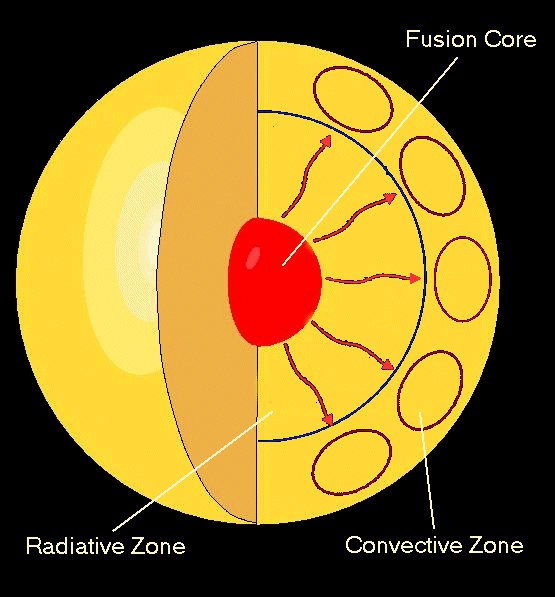
\includegraphics[scale=0.5]{working.png} 
 

\caption{Figur av konveksjon og strålings sonene i sola.} 
\end{center} 
\end{figure}

\subsection{Fremgangsmåte}
Prosjektet innebærer blant annet å løse oppgave 5.10 for å finne et uttrykk for konveksjon fluksen: 

\begin{align*}
F_C = \rho c_PT\sqrt{g\delta}H_P^{-3/2}(\frac{l_m}{2})^2(\nabla - \nabla^{\textasteriskcentered})^{3/2}
\end{align*} 

der $\nabla$ er den totale temperatur gradienten og $\nabla^{\textasteriskcentered}$ er temperatur gradienten til 
et volum av gass som har oppdrift. 

Strålingfluksen kan uttrykkes slik

\begin{align*}
F_R = \frac{4acGT^4m}{3\kappa Pr^2}\nabla
\end{align*} 

og den totale fluksen er


\begin{align*}
F_C + F_R = \frac{4acGT^4m}{3\kappa Pr^2}\nabla_{rad}
\end{align*}

Der $\nabla_{rad} $ er temeratur gradienten som trengs for at all energi blir transformert av stråling.
For å gjøre regningen videre mer oversiktlig lager jeg definisjonene 

\begin{align*}
A = \rho c_PT\sqrt{g\delta}H_P^{-3/2}(\frac{l_m}{2})^2
\end{align*} 

\begin{align*}
B = \frac{4acGT^4m}{3\kappa Pr^2}
\end{align*} 

Ved å kombinere disse uttrykkene får vi

\begin{align*}
A(\nabla - \nabla^{\textasteriskcentered})^{3/2} = B(\nabla_{rad} - \nabla)
\end{align*}

Gjennom å se på temperaturforskjellen til volumet som har oppdrift og omgivelsene får vi et uttrykk som gir oss
foskjellen mellom temperatur gradienten inne i volumet og den adiabatiske temperatur gradienten.

\begin{align*}
(\nabla^{\textasteriskcentered} - \nabla_{ad}) = \frac{32\sigma T^3}{3\kappa \rho^3c_Pv}\frac{S}{Qd}(\nabla - \nabla^{\textasteriskcentered})
\end{align*}

hvor 

\begin{align*}
v = \sqrt{\frac{g\delta l_m^2}{4H_P}}(\nabla - \nabla^{\textasteriskcentered})^{1/2}
\end{align*}

og S, d og Q er geometriske konstanter. Disse kan bli uttrykt ved $l_m $ ved radiusen til volumet

\begin{align*}
\frac{S}{Qd} = 2\frac{1}{r_P}
\end{align*} 

hvor vi antar at $r_P = \frac{1}{2}l_m $. 

\begin{align*}
\Rightarrow \frac{S}{Qd} = \frac{4}{l_m}
\end{align*} 

Ved litt triksing kan vi bruke uttrykket

\begin{align*}
(\nabla^{\textasteriskcentered} - \nabla_{ad}) = (\nabla - \nabla_{ad}) - (\nabla - \nabla^{\textasteriskcentered})
\end{align*} 

til å få en annengradsligning for $(\nabla - \nabla^{\textasteriskcentered})^{\frac{1}{2}} $, som har løsning

\begin{align*}
\xi = -\frac{2U}{l_m^2} + \sqrt{(\frac{2U}{l_m^2})^2 + (\nabla - \nabla_{ad})}
\end{align*} 

hvor

\begin{align*}
U = \frac{64\sigma T^3}{3\kappa \rho^2c_P}\sqrt{\frac{H_P}{g\delta}}
\end{align*} 

Annengradsligningen har bare en reell løsning. Siden $\xi $ er en kvadratrot må den være positiv, derav plusstegnet 
mellom leddene. Ved å sette løsningen inn i uttrykket


\begin{align*}
A(\nabla - \nabla^{\textasteriskcentered})^{3/2} = B(\nabla_{rad} - \nabla)
\end{align*}

kan vi eliminere $\nabla $ og finne konveksjon fluksen.

\begin{align*}
A\xi^3 = B(\nabla_{rad} - \nabla)
\end{align*}

\begin{align*}
\Rightarrow \nabla = \frac{B\nabla_{rad} - A\xi^3}{B} = \nabla_{rad} - \frac{A\xi^3}{B}
\end{align*}

hvor 

\begin{align*}
\nabla_{rad} = \frac{3\kappa LP}{64\pi\sigma GT^4m} = \frac{L}{4\pi r^2B}
\end{align*}

der $\sigma = \frac{ac}{4} $ er Stefan Boltzmanns konstant og A og B er som definert over.

\begin{align*}
\Rightarrow \nabla = \frac{1}{B}(\frac{L}{4\pi r^2} - A\xi^3)
\end{align*}

Ser vi tilbake på annengradsligningen $\xi $ kan vi bruke denne til å finne enda et uttrykk for $\nabla $.

\begin{align*}
\sqrt{(\frac{2U}{l_m^2})^2 + (\nabla - \nabla_{ad})} = \xi + \frac{2U}{l_m^2}
\end{align*} 

\begin{align*}
\Rightarrow \nabla = \xi^2 + \frac{4U}{l_m^2}\xi + \nabla_{ad}
\end{align*}

Setter vi disse to uttrykkene for $\nabla $ lik hverandre ender vi opp med

\begin{align*}
\Rightarrow \xi^3\frac{A}{B} + \xi^2 + \frac{4U}{l_m^2}\xi + (\nabla_{ad} - \nabla_{rad}) = 0
\end{align*}

Dette er en tredjegradsligning som kan løses
numerisk i python. Kodesnutten under løser ligningen og trekker ut den reelle løsningen. 

\begin{lstlisting}
def xieq(A, B, U, H_P, nabla_ad, nabla_rad):
	coeff = [A/B, 1, 4*U/H_P**2, (nabla_ad - nabla_rad)]
	xi = roots(coeff)
	for e in xi:
		if imag(e) == 0:
			xi = real(e) 
			break
	return xi
\end{lstlisting}


Vi har nå alt vi trenger for å finne fluksen.

\begin{align*}
F_C + F_R = \frac{4acGT^4m}{3\kappa Pr^2}\nabla_{rad}
\end{align*}

der

\begin{align*}
F_C = A\xi^3
\end{align*}

\begin{align*}
F_R = \frac{L}{4\pi r^2} - A\xi^3 
\end{align*}


Nå kan vi implementere konveksjon i modellen. Ettersom vi flytter oss gjennom stjernen gjør vi en sjekk om 
gassen er konvektiv stabil ved ustabilitets kriteriet

\begin{align*}
\nabla > \nabla_{ad}
\end{align*}

Er gassen ustabil er konveksjon den dominerende transporten. Numerisk løser jeg hvilken transportmetode som er dominerende 
slik (forkortet versjon)

\begin{lstlisting}
def konveksjon(nabla, nabla_ad):
	xi = xieq(A, B, U)	
	F_R = B*nabla
	F_C = A*xi**3
	if nabla > nabla_ad:
		F = F_C
	else:
		F = F_R
	return F
\end{lstlisting}


\subsection{Resultat}

Jeg hadde enkelte problemer i første prosjekt som har vist seg å være standhaftige. Steglengden $\partial m $ er 
fortsatt problemet, da den går mot null i rasende fart. Etter å ha skrevet om programmet, selv med hjelp fra 
mange hold, lar det seg ikke løse. Energi funksjonen viste seg ikke å være problemet, da jeg har testet den opp mot 
sanety testen og andres resultater. Koden gir meg generelt rare resultater. En kjøring der jeg gjør en sjekk om 
det enten er konveksjon eller stråling som transporterer energien, blir resultatet at stråling dominerer i 
de ytterste lagene, mens konveksjon tar over nærmere sentrum. Totalt motsatt av det man ville forvente av en vanlig 
stjerne som solen.

Utregningen av $\partial m $ i seg selv kan jeg ikke forstå at det er noe galt med.
Jeg har brukt all tiden min på dette problemet og jeg er redd jeg ikke klarer å løse det. 
Igjen uteblir resultatene til prosjektet. 

\subsection{Kode}
\begin{lstlisting}
 from numpy import *
import random
import pylab as plt



"""
Starting parameters
"""
L_0 = 3.846E26 # Luminosity [W]
R_0 = 0.5*6.96E8 # Radius [m]
M_0 = 0.7*1.989E30 # Mass [kg]
M_s = 1.989E30 # Mass sun [kg]
P_0 = 10E11 # Pressure [Pa]
ro_0 = 1E3 # Density [kg/m^3]
T_0 = 1E5 # Temperature [K]
T_c = 1.5E7*(M_0/M_s)**(1./3) #Core temperature [K]
ro_c = 1.62E5


X = 0.7 # Hydrogen
Y3 = 10**(-10) # Helium 3
Y = 0.29 # Helium 4
Z = 0.01 # Other metals
Z_Li = 10**(-13) # Lithium 7
Z_Be = 10**(-13) # Beryllium 7

m_u = 1.6605E-27 # Atomic mass unit [kg]

#my = 1./(2*X +7*Y/4 +9*Z_Be/5 +9*Z/8)# average atomic weight
my = 1./(2*X +3*Y3/3.+3*Y/4 +Z/2.)# average atomic weight
kb = 1.382E-23 # Boltzmans constant [m^2 kg/s^2 K]
c = 2.998E8 # Speed of light [m/s]
sb = 5.67E-8 # Stefan Boltzmann constant [W/m^2 K^4]
G = 6.672E-11 # Gravitaional constant [N m^2/kg^2]

Na = 6.02214129*10**23 # Avogadros konstant [1/mol]
V = 4/3*pi*R_0**3 # Volume
a = 4*sb/c

"""
#Reading the kappa values
"""

infile = open('opacity.txt', 'r')
lines = infile.readlines()
infile.close()

opacity = {}
first_line = lines[0]
logR = first_line.split()                               #the log(T) values
lgR = logR[1:]

R_list = []
for r in lgR:
	R = float(r)
        opacity[R] = {}
        R_list.append(R)


T_list = []
for line in lines[2:]:                                  #not including the first line and the blank second line
	words = line.split()
        logT =  (float(words[0]))                       #the log(T) values
        T_list.append(logT)
        kappa = words[1:]

	for r, lgk in zip(lgR, kappa):
        	opacity[float(r)][logT] = float(lgk)    #opacity[log(R)][log(T)] gives log(k)






def lamdaNa(T):
	T9 = T*1E-9		
	T9_star1 = T9/(1+4.95E-2*T9)	
	T9_star2 = T9/(1+.759*T9)

	#2xH
	l_1   = 4.01E-15*T9**(-2./3)*exp(-3.380*T9**(-1./3))*(1 +\
                     .123*T9**(1./3) + 1.09*T9**(2./3) + .938*T9)

	#2x3He
	l_2	= 6.04E10*T9**(-2./3)*exp(-12.276*T9**(-1./3))*(1 +\
                     .034*T9**(1./3) - .522*T9**(2./3)-.124*T9 + \
                     .353*T9**(4./3)+ .213*T9**(-5./3))

	#3He Be
	l_3  = 5.61E6*T9_star1**(5./6)*T9**(-3./2)*exp(-12.826*\
                     T9_star1**(-1./3))

	#Be Li
	l_4   = 1.34E-10*T9**(-1./2)*(1 - .537*T9**(1./3)  + \
                     3.86*T9**(2./3) +  .0027*T9**-1*exp(2.515E-3*T9**-1))

	#Li H
	l_5	= 1.096E9*T9**(-2./3)*exp(-8.472*T9**(-1./3)) - \
                     4.830E8*T9_star2**(5./6)*T9**(-3./2)*exp(-8.472*\
                     T9_star2**(-1./3)) + 1.06E10*T9**(-3./2)\
                     *exp(-30.442*T9**-1)

	return l_1, l_2, l_3, l_4, l_5





def efunk(ro, T, mu):
	# Densities of atomic species
	n_p = ro*X/(1.*mu)
	n_He = ro*Y/(4.*mu)
	n_e = (ro/2.*mu)*(1. + X)
	n_d = ro*X/(2.*mu)
	n_3He = ro*Y3/(3.*mu)
	n_Li = ro*Z_Li/(7.*mu)
	n_Be = ro*Z_Be/(7.*mu)

	
	[l_1, l_2, l_3, l_4, l_5] = lamdaNa(T)

	#complete lambda functions
	lm_1 = l_1/Na#*1E-6
	lm_2 = l_2/Na#*1E-6
	lm_3 = l_3/Na#*1E-6
	lm_4 = l_4/Na#*1E-6
	lm_5 = l_5/Na#*1E-6


	#reaktion rates
	r_pp = n_p**2/(ro*2)*lm_1
	r_pd = r_pp
	r_33 = n_3He**2  /(ro*2)*lm_2
	r_34 = n_3He*n_He/ro*lm_3
	r_e7 = n_Li*n_Be/ro*lm_4
	r_71 = n_Li*n_p/ro*lm_5

	#Check and correct for reactions that overstep their fuel
	if 2.*r_33 + r_34 > r_pd:
		r_33 = 2./3*r_pd
		r_34 = 1./3*r_pd
	if r_e7 > r_34:
		r_e7 = r_34
	if r_71 > r_e7:
		r_71 = r_e7

	
	# free energy
	Q1 = 0.15E6*1.602176565E-19 
	Q2 = 5.49E6*1.602176565E-19 
	Q3 = 12.86E6*1.602176565E-19
	Q4 = 1.59E6*1.602176565E-19
	Q7e = 0.05E6*1.602176565E-19
	Q71 = 17.35E6*1.602176565E-19

	# full energy
	e_1 = r_pp*(Q1+Q2)
	e_2 = r_33*Q3
	e_3 = r_34*Q4
	e_4 = r_e7*Q7e
	e_5 = r_71*Q71
	
	
	E = e_1+e_2+e_3+e_4+e_5
	return e_1, e_2, e_3, e_4, e_5






def xieq(A, B, U, H_P, nabla_ad, nabla_rad):
	coeff = [A/B, 1, 4*U/H_P**2, (nabla_ad - nabla_rad)]
	xi = roots(coeff)
	for e in xi:
		if imag(e) == 0:
			xi = real(e) 
			break
	return xi





def konveksjon(T, P, r, M, ro, k_SI, mu, L, convection, radiation):


	delta = 1.
	alpha = 1.
	g = 274.
	c_P = 1.
	m = 1.
	N = m/(my*mu)

	H_P = (1./3)*(3.*N*kb*T/(4.*pi*P))**(1/3)
	l_m = alpha*H_P


	A = ro*c_P*T*sqrt(g*delta)*H_P**(-3./2)*(l_m/2.)**2
	B = 16*sb*G*T**4*M/(3*k_SI*P*r**2)
	U = 64.*sb*T**3/(3.*k_SI*ro**2.*c_P)*sqrt(H_P/(g*delta))


	#print A
	#print B
	#print U

	nabla_rad = L/(4.*pi*r**2*B)
	nabla_ad = P*delta/(T*ro*c_P)
		
	xi = xieq(A, B, U, H_P, nabla_ad, nabla_rad)
	#print xi

	nabla = 1./B*(L/(4*pi*r**2) - A*xi**3)
	nabla_s = nabla_rad - (A/B)*xi**3

		

	F_R = B*nabla

	F_C = A*xi**3
	
	if nabla > nabla_ad:
		F = F_C
		convection.append(1)
		#print 'convection'
	else:
		F = F_R
		#print 'radiation'
		radiation.append(1)
	return F



n = 10000

def evolution(r, ro, m, T, mu):
	
	r = zeros(n)	
	r[0] = 0.5*6.96E8
	P = zeros(n)
	#P[0] = P_0
	
	L = zeros(n)
	L[0] = 3.846E26
	T = zeros(n)
	T[0] = 5770.
	M = zeros(n)
	E_list = zeros(n)

	ro1 = 4.0E-4
	P[0] = ro1*kb*T[0]/(my*mu)
	M[0] = M_0

	convection = []
	radiation = []

	cnt = []
	ro_list = []
	ro_list.append(P_0*my*mu/(sb*T_0))
	dm_list2 = zeros(n)
	

	E_list = []
	E_list.append(0)

	PP1 = zeros(n)
	PP2 = zeros(n)

	e1 = zeros(n)
	e2 = zeros(n)
	e3 = zeros(n)	
	e4 = zeros(n)
	e5 = zeros(n)


	for i in range(n-1):
		counter = 1
		cnt.append(counter)
		
		ro = P[i]*my*mu/(sb*T[i])
		ro_list.append(ro)
	
		#print 'ro = %.4g' % (ro)




		#Opacity
		logR = log10(ro*10**(-3)*10**6/T[i])
		logT = log10(T[i])
		LogR = min(R_list, key=lambda x:abs(x-logR))
		LogT = min(T_list, key=lambda x:abs(x-logT)) 

		lgk = float(opacity[LogR][LogT])                               
		k_SI = 10**(lgk-1)

		#print k_SI
		
        	#BVG :: HER KOMMER kappa UT I CGS ENHETER...... DU MAA HER
        	#         KONVERTERE ENHETEN FOR kappa FRA CGS TIL SI
		
		k_SI = k_SI*1E-4/1E-3




		# Energy
		[e_1, e_2, e_3, e_4, e_5] = efunk(ro, T[i], m_u)
		E = e_1+e_2+e_3+e_4+e_5		
		E_list.append(E)
		
		e1[i] = e_1
		e2[i] = e_2
		e3[i] = e_3
		e4[i] = e_4
		e5[i] = e_5





		#finding dm
		dm_list = []


		dr_dm = 1./(4*pi*r[i]**2*ro)
		dP_dm = - G*M[i]/(4*pi*r[i]**4)
		dL_dm = E
		dT_dm = -3.*k_SI*L[i]/(256.*pi**2*sb*r[i]**4*T[i]**3)
		
		#print 'dr_dm = %.g' % (dr_dm)
		#print 'dP_dm = %.g' % (dP_dm)
		#print 'dT_dm = %.g' % (dT_dm)
		#print 'dL_dm = %.g' % (dL_dm)	
		
		P_r = (1./3)*a*T[i]**4 

		f1 = dr_dm
		dm1 = abs(r[i]*0.01/f1)
		#print 'dm1 = %.4g' % (dm1)
		dm_list.append(dm1)

		f2 = dP_dm
		dm2 = abs(P[i]*0.01/f2)
		#print 'dm2 = %.4g' % (dm2)
		dm_list.append(dm2)

		f3 = dL_dm
		dm3 = abs(L[i]*0.01/f3)
		#print 'dm3 = %.4g' % (dm3)
		dm_list.append(dm3)

		f4 = dT_dm
		dm4 = abs(T[i]*0.01/f4)
		#print 'dm4 = %.4g' % (dm4)
		dm_list.append(dm4)

		dm = -min(dm_list)
		dm_list2[i] = dm		

		#print 'dm = %.4g' % (dm)





		# Integrating
		M[i+1] = M[i] + dm

		if M[i+1] < 0:
			break


		r[i+1] = dr_dm*dm + r[i]

		P[i+1] = dP_dm*dm + P_r + P[i]
		
		L[i+1] = dL_dm*dm + L[i]

		T[i+1] = dT_dm*dm + T[i]

		#print 'r = %.g' % (r[i])
		#print 'P = %.g' % (P[i])
		#print 'L = %.g' % (L[i])
		#print 'T =%.g' % (T[i])
		#print 'M = %.4g'% (M[i])

		#print dr_dm/r[i]
		#print r[i]/r[0]		

		F = konveksjon(T[i], P[i], r[i], M[i], ro, k_SI, mu, L[i], convection, radiation)
	



	#PP1 and PP2 chain
	for j in range(n):
		PP1[j] = e1[j]*0.69 + e2[j]
		PP2[j] = e1[j]*0.31 + e3[j] + e4[j] + e5[j]



	print size(cnt)
	return r, P, L, T, M, dm_list2, ro_list, convection, radiation, F, PP1, PP2, E_list




r, P, L, T, M, dm, ro, convection, radiation, F, PP1, PP2, E_list = evolution(R_0, ro_0, M_0, T_0, m_u)



#plt.plot(r, PP2)
#plt.plot(P,r)
#plt.title(['Radius/dm'])
#plt.axes(['dm', 'r'])
#plt.show()
\end{lstlisting}



\end{document}